\chapter{TINJAUAN PUSTAKA}
\label{chap:tinjauanpustaka}

% Ubah bagian-bagian berikut dengan isi dari tinjauan pustaka

\section{Hasil penelitian terdahulu}
\subsection{Pengembangan Sistem Deteksi Kantuk Menggunakan Pengklasifikasi \emph{Random Forest} pada Sinyal Elektrokardiogram}
Pada penelitian ini Nuryani Nuryani, Khoirun Nisak, Artono Dwijo Sutomo mengembangkan   sistem   deteksi   kantuk
memakai   sinyal elektrokardiogram  (EKG)  dan \emph{Random  Forest}. Sistem  deteksi kantuk   dilatih   memakai suatu
rekaman   EKG   dari database DROZY yang dilengkapi \emph{Karolinska Sleepiness Scale}(KSS). Fitur masukan  sistem  diekstraksi
bersumberkan pada  metode ranah waktu serta ranah frekuensi \parencite{9}.

\subsection{Deteksi Kantuk Berdasarkan Pola Bukaan Mulut Menggunakan Metode 1D CNN}
Pada penelitian ini Victorio Valendion melakukan riset tentang deteksi kantuk memakai landmark bagian mulut melalui
memperhitungkan pola dari terbuka serta tertutup-nya mulut. Nilai dari rasio bukaan mulut dihitung selanjutnya
semua data nya disimpan ke dalam suatu file csv yang kemudian akan dilakukan proses pelatihan untuk mesin
supaya dapat mendeteksi kantuk dengan arsitektur 1D CNN \parencite{10}.

\subsection{Klasifikasi Skala Kantuk Karolinska Berdasarkan Nilai \emph{Eye Aspect Ratio} Menggunakan \emph{Deep Learning}}
Pada penelitian ini Annida Miftakhul Farodisa melakukan riset tentang deteksi kantuk menggunakan metode non-intrusif
dengan memanfaatkan kamera (fitur wajah) dan \emph{deep learning}. Penulis membuat model klasifikasi Skala Kantuk Karolinska
(KSS) berdasarkan nilai \emph{Eye Aspect Ratio}. Penelitian ini menggunakan video \emph{near-infrared} NIR pada dataset DROZY yang berisi video
subjek saat menjalani pengujian kewaspadaan psikomotorik yang mengisi kuesioner Skala Kantuk Karolinska (KSS) sebelum
memulai pengujian. Dilakukan ekstraksi nilai EAR untuk setiap subjek pada setiap frame di setiap video sehingga
membentuk pola EAR dan dilabeli dengan KSS yang dikelompokkan menjadi empat kelas \parencite{11}.

\subsection{Deteksi Kantuk Pada Pengendara Roda Empat Melalui Citra Wajah Menggunakan Metode \emph{Facial Landmark}}
Pada penelitian ini Muhammad Akbar Maulana melakukan riset tentang deteksi kantuk pada pengendara roda empat melalui
citra wajah memakai metode facial landmark. Membuat suatu sistem yang bisa memperingatkan pengemudi secara otomatis
jika pengemudi memperlihatkan gejala mengantuk ketika mengendarai kendaraan akhirnya diharapkan bisa mengurangi
resiko kecelakaan yang bisa terjadi kepada pengendara tersebut. Guna menetapkan pengendara mengantuk ataupun tidak
sistem ini menggunakan algoritma \emph{regression trees} dengan mengambil 2 parameter (\emph{eye blink and Mouth detector}) \parencite{12}.

\section{\emph{Library} Dlib}

Dlib merupakan library open source populer dalam bidang computer vision dan
machine learning. Dlib menyediakan berbagai algoritma dan fungsi yang berguna untuk
berbagai tugas seperti deteksi objek, pengenalan wajah, estimasi pose, deteksi landmark,
pengolahan citra, dan lainnya. Dlib dapat berjalan di berbagai platform seperti Windows,
macOS, Linux, dan Android \parencite{14}. Algoritma deteksi wajah Dlib menggunakan
metode Histogram of Oriented Gradients (HOG) yang dikombinasikan dengan Support Vector
Machines (SVM) untuk menghasilkan deteksi yang akurat. Dlib memiliki kemampuan untuk mendeteksi landmark pada wajah,
yaitu titik-titik penting seperti mata, hidung, dan mulut. Deteksi landmark ini berguna
dalam berbagai aplikasi seperti estimasi pose wajah, analisis ekspresi wajah, dan
penerapan makeup virtual.

\section{\emph{Facial Landmark}}
\emph{Facial Landmark} merupakan ekstraksi titik-titik pada wajah yang tersebar menggunakan detektor wajah \parencite{15}.  Pendeteksi
\emph{facial landmark} diaplikasikan ke \emph{input frames} untuk mendeteksi fitur wajah dengan menggunakan \emph{library} dlib yang
menggunakan \emph{Histogram Oriented Gradients} (HOG) untuk pendeteksian wajah dan \emph{Linear Support Vector Machine} (SVM)
sebagai \emph{classifier} dalam prosedur pengenalan landmark wajah \parencite{16}. Terdapat 68 titik yang merepresentasikan wajah,
titik koordinat tersebut merepresentasikan fitur sesuai dengan gambar \ref{fig:wajah}:

\begin{figure} [H] \centering
  % Nama dari file gambar yang diinputkan
  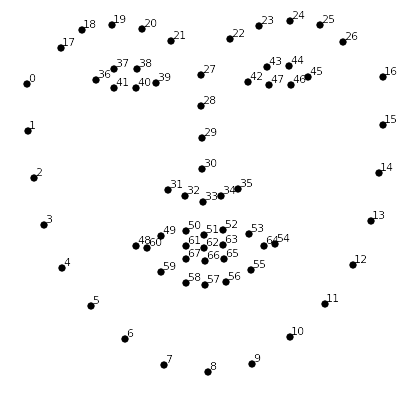
\includegraphics[scale=0.75]{gambar/wajah.png}
  % Keterangan gambar yang diinputkan
  \caption{Landmark wajah manusia \parencite{16}}
  % Label referensi dari gambar yang diinputkan
  \label{fig:wajah}
\end{figure}

1.	Dagu		: 0-16

2.	Alis kanan	: 17-21

3.	Alis kiri		: 22-26

4.	Hidung		: 27-35

5.	Mata kanan	: 36-41

6.	Mata kiri	: 42-47

7.	Mulut		: 48-60

8.	Bibir		: 61-67

\subsection{\emph{Eye Aspect Ratio} (EAR)}
EAR merupakan salah satu metode yang dapat digunakan untuk bisa menghitung jarak antara kelopak mata atas serta
kelopak mata bawah bersumberkan titik geometri wajah pada mata. Metode EAR ini selalu dipergunakan untuk menghitung
pola bukaan mata individual setiap menitnya. Perhitungan EAR ini dihitung bersumberkan pada koordinat mata kiri serta
kanan yang ada dalam landmark wajah. EAR pada landmark wajah bisa diilustrasikan denggan gambar \ref{fig:mata} :

\begin{figure} [H] \centering
  % Nama dari file gambar yang diinputkan
  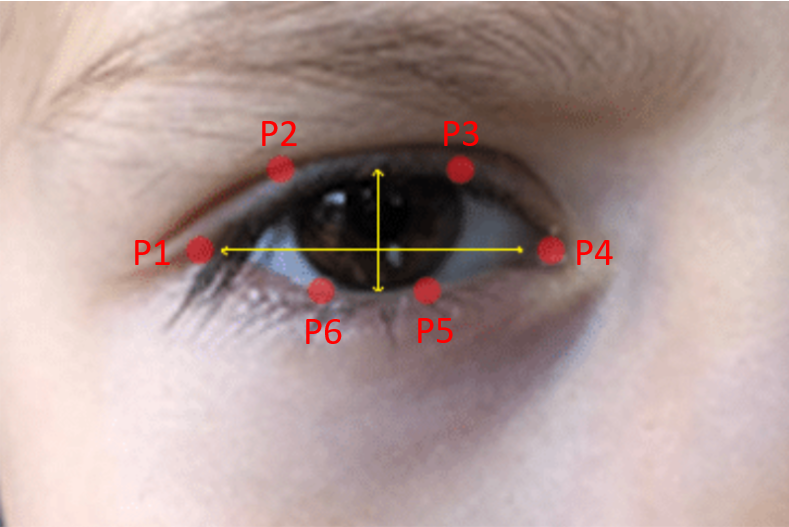
\includegraphics[scale=0.35]{gambar/mata.png}
  % Keterangan gambar yang diinputkan
  \caption{enam titik landmark pada mata \parencite{20}}
  % Label referensi dari gambar yang diinputkan
  \label{fig:mata}
\end{figure}

Nilai EAR didapati dari menghitung jarak antara kelopak mata yang didapatkan melalui mengambil titik tepat ditengah
kelopak mata atas serta kelopak mata bawah. Rumus tersebut dapat dituliskan sesuai rumus \ref{eq:EAR}:

% Contoh pembuatan persamaan
\begin{equation}
  % Label referensi dari persamaan yang dibuat
  \label{eq:EAR}
  % Baris kode persamaan yang dibuat
  EAR = \frac{\left \| P2-P6 \right \| + \left \| P3-P5 \right \|}{2 \left \| P1-P4 \right \|}
\end{equation}

Ketika mata berkedip, dibutuhkan 100 - 400 ms untuk menutup. Perihal ini diperkuat oleh penelitian yang diselengarakan
oleh Caffier et al., yang menyatakan bahwasanya mata tertutup membutuhkan sekitar 200 ms. Sedangkan saat mengantuk,
mata membutuhkan lebih dari 500 ms untuk menutup. Itu perkiraan mata tertutup dimulai saat mata mulai menutup sampai
sepenuhnya tertutup \parencite{17}.

\subsection{\emph{Mouth Aspect Ratio} (MAR)}
MAR ialah salah satu metode yang dapat dipergunakan untuk dapat menghitung jarak antara bibir atas dan bibir bawah
bersumberkan titik geometri wajah pada mulut. Metode MAR ini selalu dipakai guna menghitung bukaan mulut seseorang \parencite{12}.
MAR pada landmark wajah bisa diilustrasikan dengan gambar \ref{fig:mulut} :

\begin{figure} [H] \centering
  % Nama dari file gambar yang diinputkan
  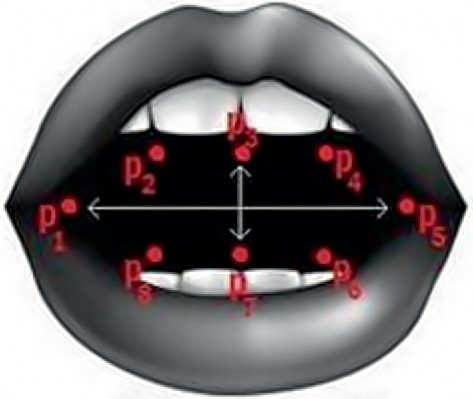
\includegraphics[scale=0.4]{gambar/mulut.png}
  % Keterangan gambar yang diinputkan
  \caption{Enam titik landmark pada mulut \parencite{21}}
  % Label referensi dari gambar yang diinputkan
  \label{fig:mulut}
\end{figure}

Perhitungan nilai MAR sama dengan perhitungan nilai EAR yaitu dengan menghitung jarak antara bibir yang diambil dengan
mengambil titik tepat ditengah bibir atas dan bibir bawah. Rumus tersebut dapat dituliskan menjadi rumus \ref{eq:MAR}:

\begin{equation}
  % Label referensi dari persamaan yang dibuat
  \label{eq:MAR}
  % Baris kode persamaan yang dibuat
  MAR = \frac{\left \| P2-P8 \right \| + \left \| P3-P7 \right \| + \left \| P4-P6 \right \|}{3 \left \| P1-P5 \right \|}
\end{equation}

\section{Skala Kantuk Karolinska(KSS)}
Skala Kantuk Karolinska menjadi alat yang paling banyak digunakan untuk perhitungan kewaspadaan dalam investigasi
kronobiologis dan tidur. KSS ditemukan menjadi pengukur kantuk yang andal dan sensitif (Gillberg et al., 1994), dan
itu divalidasi oleh beberapa pengukuran fisiologis yang berbeda (Kaida et al., 2006; Marzano et al., 2007; Filtness
et al., 2021). Untuk mendeteksi transisi antara terjaga dan tidur dapat diukur menggunakan indeks fisiologis
sederhana yang diambil dan ditentukan dari rekaman \emph{electroencephalogram} (EEG). Nilai pada KSS berkisar antara 1
(amat sangat terjaga) hingga 9 (sangat mengantuk, berusaha lebih untuk terjaga) \parencite{19}. Hal tersebut dapat
digambarkan menjadi seperti tabel \ref{tbl:Skala}:

\begin{table}[h!]
  \centering
  \caption{Tabel Skala Kantuk Karolinska \parencite{19}}
  \begin{tabular}{|p{1.5cm} |c|}

    \hline
    Skala & Tingkat Kantuk/Keterjagaan                     \\
    \hline

    % Gunakan \G untuk mengisi sel dan \w untuk mengosongkan sel
    1     & Amat Sangat Terjaga                            \\
    \hline

    2     & Sangat Terjaga                                 \\
    \hline

    3     & Terjaga                                        \\
    \hline

    4     & Sedikit Terjaga                                \\
    \hline

    5     & Tidak Terjaga namun Tidak ada tanda Mengantuk  \\
    \hline

    6     & Sedikit Mengantuk                              \\
    \hline

    7     & Mengantuk, sedikit usaha untuk Terjaga         \\
    \hline

    8     & Mengantuk, perlu usaha untuk Terjaga           \\
    \hline

    9     & Sangat Mengantuk, berusaha lebih untuk Terjaga \\
    \hline
  \end{tabular}
  \label{tbl:Skala}
\end{table}

\section{Interpolasi Data}

Interpolasi dilakukan untuk mengisi atau memperkirakan nilai yang hilang atau
tidak tersedia dalam dataset dengan menggunakan teknik-teknik yang sesuai. Dalam
beberapa kasus, dataset yang dikumpulkan mungkin tidak lengkap atau terdapat
kehilangan data pada beberapa fitur. \parencite{24}. Beberapa teknik interpolasi
data yang umum digunakan dalam machine learning meliputi:

\begin{enumerate}[nolistsep]
  \item Interpolasi Linear: Teknik ini melibatkan estimasi nilai yang hilang berdasarkan
        hubungan linear antara titik data yang diketahui. Interpolasi linear digunakan
        jika data memiliki hubungan linier yang jelas antara fitur-fitur yang terlibat.

  \item Interpolasi Nearest Neighbor: Metode ini mengisi nilai yang hilang dengan
        menggunakan nilai terdekat dari data terdekat dalam dataset.
        data terdekat dapat ditentukan berdasarkan jarak Euclidean atau metode lainnya.

  \item Interpolasi Polinomial: Metode ini melibatkan pendekatan fungsi polinomial
        untuk mengisi nilai yang hilang. Polinom dapat disesuaikan dengan data yang tersedia
        untuk memperkirakan nilai yang hilang.

  \item Interpolasi Kriging: Teknik ini merupakan metode stokastik yang menggunakan
        model spasial untuk memprediksi nilai yang hilang berdasarkan korelasi spasial antara
        data yang diketahui.

  \item Interpolasi Regresi: Pendekatan ini melibatkan penggunaan model regresi untuk
        memperkirakan nilai yang hilang berdasarkan hubungan antara atribut-atribut yang
        tersedia.
\end{enumerate}

\section{Normalisasi}

Normalisasi dadalah proses mengubah skala nilai dari fitur-fitur dalam dataset
agar memiliki distribusi data yang seragam atau terstandarisasi. Tujuan normalisasi
adalah untuk memastikan bahwa fitur-fitur dengan skala yang berbeda memiliki pengaruh
yang sebanding terhadap proses pembelajaran algoritma \parencite{25}. Beberapa metode
normalisasi umum digunakan adalah sebagai berikut:

\begin{enumerate}[nolistsep]
  \item Min-Max Scaling: Metode ini mentransformasikan setiap nilai fitur menjadi r
        entang yang ditentukan, biasanya antara 0 dan 1. Rumus umum untuk melakukan
        normalisasi Min-Max Scaling adalah sebagai berikut:
        \begin{equation}
          % Label referensi dari persamaan yang dibuat
          \label{eq:MinMax}
          % Baris kode persamaan yang dibuat
          X' = \frac{X - Xmin}{Xmax - Xmin}
        \end{equation}
        Pada rumus \ref{eq:MinMax} X merupakan nilai asli, X' merupakan nilai yang telah
        dinormalisasi, Xmin adalah nilai minimum yang ada pada dataset, dan Xmax adalah nilai
        maksimum yang ada pada dataset.

  \item Z-Score Scaling: Metode ini mengubah nilai fitur menjadi distribusi standar
        dengan mean (rata-rata) 0 dan standard deviation (deviasi standar) 1. Rumus umum
        untuk melakukan normalisasi Z-Score Scaling adalah sebagai berikut:
        \begin{equation}
          % Label referensi dari persamaan yang dibuat
          \label{eq:StandardScaler}
          % Baris kode persamaan yang dibuat
          X' = \frac{X - mean}{stdDev}
        \end{equation}
        Pada rumus \ref{eq:StandardScaler} X merupakan nilai asli, X' merupakan nilai yang telah
        dinormalisasi, mean merupakan nilai rata-rata fitur yang ada pada dataset, dan stdDev
        merupakan nilai standar deviasi dari fitur yang ada pada dataset.
\end{enumerate}

\newpage
\section{\emph{Deep Learning}}
\emph{Deep Learning} memungkinkan model komputasi yang memuat atas sejumlah lapisan pemrosesan guna memahami representasi data
melalui sejumlah tingkatan abstraksi. Metode-metode ini sudah meningkatkan \emph{state-of-the-art} dalam pengenalan suara,
pengenalan objek visual, deteksi objek serta banyak domain lainnya secara dramatis. \emph{Deep Learning} mendapati struktur
rumit dalam kumpulan data besar yang memakai algoritma backpropagation guna memperlihatkan bagaimana mesin perlu merubah
parameter internalnya yang dipakai guna memperhitungkan representasi di setiap lapisan dari representasi di lapisan
sebelumnya. \emph{Deep Convolutional Network} mendapatkan terobosan dalam pemrosesan gambar, video, ucapan, serta audio,
sementara \emph{Recurrent Neural Network} menyoroti data berurutan berupa teks serta ucapan \parencite{18}.

\section{\emph{Recurrent Neural Network} (RNN)}

\begin{figure} [H] \centering
  % Nama dari file gambar yang diinputkan
  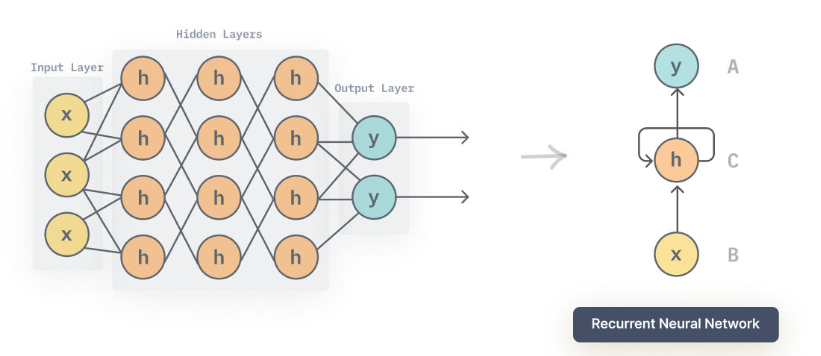
\includegraphics[scale=0.55]{gambar/rnn.png}
  % Keterangan gambar yang diinputkan
  \caption{Ilustrasi RNN \parencite{18}}
  % Label referensi dari gambar yang diinputkan
  \label{fig:rnn}
\end{figure}

Untuk tugas yang melibatkan input berurutan, seperti ucapan dan bahasa, seringkali lebih baik untuk menggunakan RNN.
RNN mempunyai memori yang bisa dipergunakan untuk menyimpan state, memori ini memungkinkan RNN untuk memiliki pemahaman
tentang konteks sebelumnya saat memproses langkah berikutnya. RNN memproses urutan input satu elemen pada setiap waktu,
mempertahankan di unit tersembunyi mereka sebuah \emph{state vektor} yang secara implisit berisi informasi tentang sejarah semua
elemen masa lalu dari urutannya yang bisa diilustrasikan dengan gambar \ref{fig:rnn}.

RNN menggunakan bobot yang bersama-sama digunakan di setiap langkah, dengan tujuan menghasilkan pembaruan yang konsisten
pada setiap langkah. Bobot ini mencerminkan hubungan antara langkah sebelumnya dan langkah berikutnya.Ketika kita
mempertimbangkan output dari unit tersembunyi di langkah-langkah waktu diskrit yang berbeda seolah-olah mereka adalah output
dari yang berbeda neuron dalam \emph{deep multilayer network}. Backpropagation digunakan untuk melatih RNN dengan menghitung gradien
kesalahan melalui setiap langkah waktu dan memperbarui bobot-bobot berdasarkan gradien tersebut. Hal ini memungkinkan RNN untuk
belajar dan menyesuaikan diri dengan pola dalam data urutan.\parencite{18}.

\newpage

\section{\emph{Independent RNN} (IndRNN)}

\begin{figure} [H] \centering
  % Nama dari file gambar yang diinputkan
  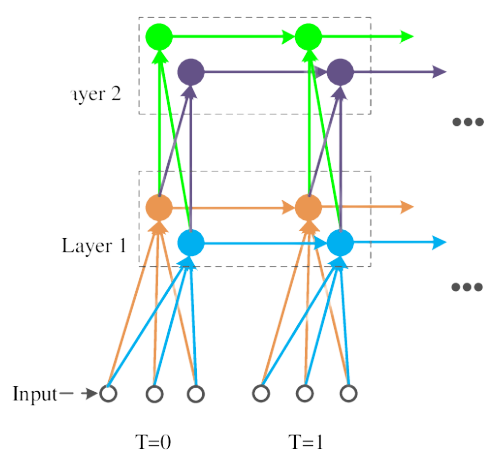
\includegraphics[scale=0.45]{gambar/indrnn.png}
  % Keterangan gambar yang diinputkan
  \caption{Ilustrasi IndRNN \parencite{8}}
  % Label referensi dari gambar yang diinputkan
  \label{fig:indrnn}
\end{figure}

IndRNN merupakan salah satu variasi \emph{deep learning} hasil pengembangan RNN yang bisa mengetahui pola temporal. IndRNN ini
diperlihatkan oleh Shuali Li et al. (2019). IndRNN memperkenalkan gagasan independensi di antara unit-unit waktu dalam jaringan rekuren,
sehingga setiap unit rekuren dapat beroperasi secara mandiri tanpa ketergantungan langsung pada unit-unit sebelumnya atau sesudahnya.
sedangkan pada RNN, setiap neuron terkait satu dengan lainnya dalam satu layer sesuai gambar \ref{fig:indrnn}. Pemrosesan neuron yang
independen ini memungkinkan IndRNN untuk memproses urutan panjang dengan menggunakan parameter yang sama pada setiap unit rekuren.
Keunggulan IndRNN terletak pada kemampuannya untuk memproses urutan waktu yang panjang dengan menggunakan parameter yang lebih efisien
dan menghindari \emph{vanishing gradient problem} yang sering terjadi pada RNN tradisional.



\section{\emph{Long Short Terms Memory} (LSTM)}

\begin{figure} [H] \centering
  % Nama dari file gambar yang diinputkan
  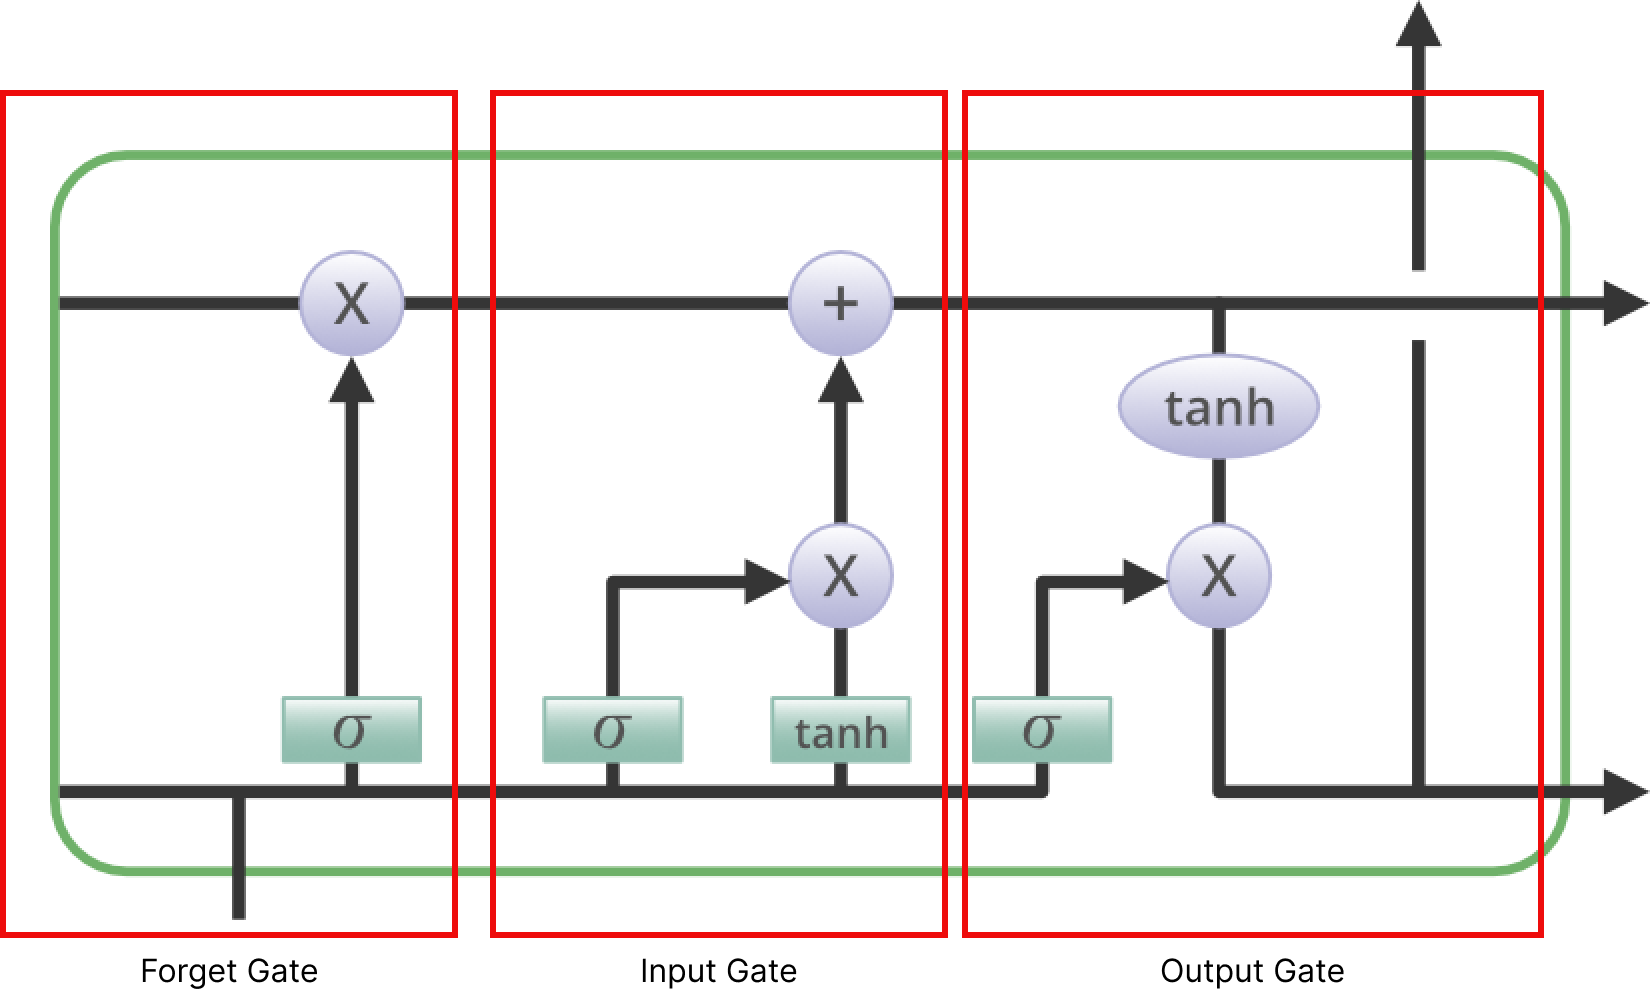
\includegraphics[scale=0.2]{gambar/LSTM.png}
  % Keterangan gambar yang diinputkan
  \caption{Struktur LSTM}
  % Label referensi dari gambar yang diinputkan
  \label{fig:LSTM}
\end{figure}

LSTM merupakan pengembangan atau salah satu jenis dari algoritma RNN
(\emph{Recurrent Neural Network}) yaitu dengan menambahkan memory cell yang dapat menyimpan
informasi untuk jangka waktu yang lama \parencite{26}. LSTM diajukan sebagai solusi
untuk mengatasi masalah \emph{vanishing gradient} yang terjadi saat memproses data berurutan
yang panjang saat menggunakan RNN. LSTM memiliki kemampuan untuk mengingat informasi
yang telah disimpan dalam jangka waktu panjang dan menghapus informasi yang tidak
relevan sehingga memungkinkannya untuk lebih efisien memproses, memprediksi, dan mengklasifikasikan
data berdasarkan urutan waktu tertentu. LSTM juga melibatkan proses backpropagation untuk melatih dan
memperbarui bobot-bobotnya. Gradien dihitung mundur melalui waktu untuk memperbarui bobot-bobot secara efisien.

Sistem LSTM terdiri dari empat gerbang, yaitu masukan (\emph{input gate}), gerbang
lupa (\emph{forget gate}), gerbang dan gerbang keluaran (\emph{output gate}) \parencite{27}.
Setiap gerbang memiliki peran dan tugasnya sendiri dalam mengumpulkan,
mengklasifikasi, dan memproses data. Selain memiliki empat gerbang tersebut,
LSTM juga dilengkapi dengan sel memori internal. Berikut penjelasan rinci mengenai komponen-komponen
pada LSTM:

\begin{enumerate}[nolistsep]
  \item Gerbang Input (\emph{Input Gate})

        Gerbang input mengontrol seberapa banyak informasi baru harus
        dimasukkan ke dalam sel memori. Ini melibatkan penggunaan fungsi
        aktivasi sigmoid untuk menghasilkan vektor bobot yang memperkirakan
        tingkat pentingnya informasi baru.

  \item Gerbang Lupa (\emph{Forget Gate})

        Gerbang lupa menentukan seberapa banyak informasi lama dalam sel
        memori harus dilupakan. Ini juga menggunakan fungsi aktivasi sigmoid
        untuk menghasilkan vektor bobot yang menentukan sejauh mana informasi
        lama harus dihapus atau dipertahankan.

  \item Sel Memori

        Sel memori merupakan komponen sentral dalam LSTM. Ini berfungsi
        sebagai "memori" jangka panjang yang dapat menyimpan dan mengingat
        informasi dalam urutan data. Sel memori dikontrol oleh gerbang input
        dan gerbang lupa untuk memperbarui dan mempertahankan informasi yang
        relevan.

  \item Gerbang Keluaran (\emph{Output Gate})

        Gerbang keluaran mengatur sejauh mana informasi dalam sel memori harus
        diungkapkan ke luar. Fungsi aktivasi sigmoid digunakan untuk menghasilkan
        vektor bobot yang mengontrol jumlah informasi yang dilewatkan.
\end{enumerate}

\section{\emph{Support Vector Machine} (SVM)}

\begin{figure} [H] \centering
  % Nama dari file gambar yang diinputkan
  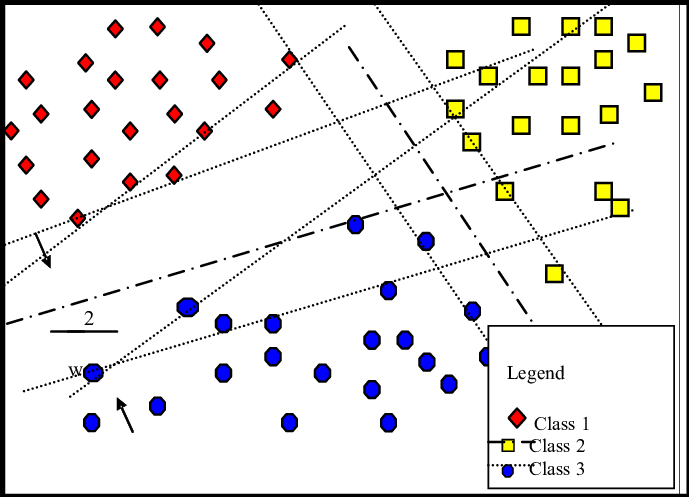
\includegraphics[scale=0.35]{gambar/SVM.png}
  % Keterangan gambar yang diinputkan
  \caption{SVM multiklas}
  % Label referensi dari gambar yang diinputkan
  \label{fig:SVM}
\end{figure}

SVM (\emph{Support Vector Machine}) adalah sebuah algoritma pembelajaran mesin yang
digunakan untuk tugas klasifikasi dan regresi. SVM menciptakan sebuah
hiperplane atau sebuah garis pemisah yang optimal dalam ruang fitur untuk
memisahkan data menjadi kelas yang berbeda. \parencite{28}

\begin{enumerate}[nolistsep]
  \item Klasifikasi Linear:

        SVM memiliki kemampuan untuk melakukan klasifikasi linear, di mana
        algoritma ini mencari hiperplane yang secara optimal memisahkan dua kelas
        data. Hiperplane tersebut dapat berupa garis atau bidang yang berfungsi
        sebagai pemisah. SVM berupaya menemukan hiperplane dengan margin terbesar
        di antara dua kelas, yaitu jarak terpendek antara hiperplane dan titik-titik
        data terdekat dari masing-masing kelas.

  \item Kernel:

        SVM juga memiliki kemampuan untuk memodelkan hubungan non-linear antara
        fitur-fitur dengan menggunakan kernel. Kernel merupakan suatu fungsi
        yang mengubah data ke dalam ruang fitur yang memiliki dimensi lebih
        tinggi. Dalam ruang fitur yang lebih tinggi tersebut, SVM mencari
        hiperplane linier yang mampu memisahkan data secara optimal. Beberapa
        jenis kernel yang sering digunakan meliputi kernel linier, kernel
        polinomial, dan kernel radial basis function (RBF).

  \item Support Vectors:

        Support vectors adalah titik-titik data yang terletak pada atau dekat
        hiperplane pembatas. SVM menggunakan support vectors ini untuk
        menentukan hiperplane yang optimal. Hanya support vectors yang
        mempengaruhi posisi dan bentuk hiperplane, sementara titik-titik data
        lainnya tidak berperan dalam pembentukan hiperplane.

  \item Regularisasi dan Penalti:

        SVM menerapkan konsep regularisasi untuk mencegah overfitting.
        Parameter C dalam SVM mengatur keseimbangan antara mencapai margin
        maksimum dan mengurangi jumlah pelanggaran batas pemisah
        (misclassification). Semakin besar nilai C, semakin besar penalti
        yang diberikan untuk pelanggaran batas pemisah. Dengan demikian,
        nilai C yang lebih tinggi cenderung menghasilkan model yang lebih
        ketat dengan margin yang lebih sempit, sementara nilai C yang lebih
        rendah dapat memungkinkan adanya pelanggaran batas pemisah yang lebih
        besar.

  \item Regresi:

        Selain untuk klasifikasi, SVM juga dapat diterapkan dalam tugas
        regresi. Dalam SVM regresi, tujuannya adalah untuk membangun sebuah
        model yang dapat mendekati fungsi target dengan cara meminimalkan
        kesalahan antara output model dan target sebanyak mungkin. SVM regresi
        berusaha untuk menciptakan sebuah hiperplane yang memiliki margin
        terbesar di sekitar titik-titik data yang ada.
\end{enumerate}
